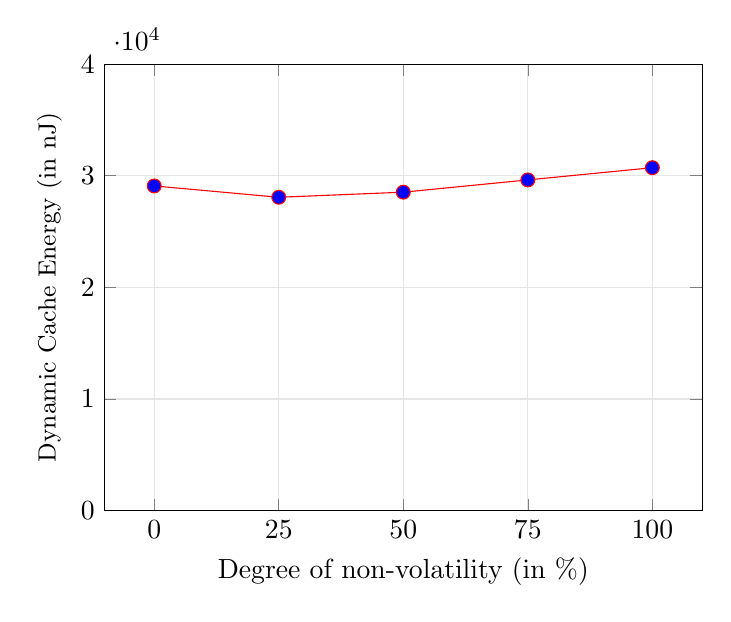
\begin{tikzpicture}
 
\begin{axis}[
	xmin = -10,
	xmax = 110,
	xtick distance = 25,
	ymin = 0,
	ymax = 40000,
	ytick distance = 10000,
    grid = both,
    major grid style = {gray!20},
    width = \columnwidth,
    height = 0.78\textwidth,
    xlabel = { \normalsize Degree of non-volatility (in \%)},
    ylabel = {\small Dynamic Cache Energy (in nJ)},
    scale = 0.72
    ]

\addplot[red,mark=*,mark options={scale=1.25, fill=blue},text mark as node=true,point meta=explicit symbolic] coordinates { (0,29088.925748) (25,28074.614715) (50,28530.362257) (75,29628.430611) (100,30723.784948)};

\end{axis}
\end{tikzpicture}